\documentclass[svgnames,tikz]{standalone}




\begin{document}
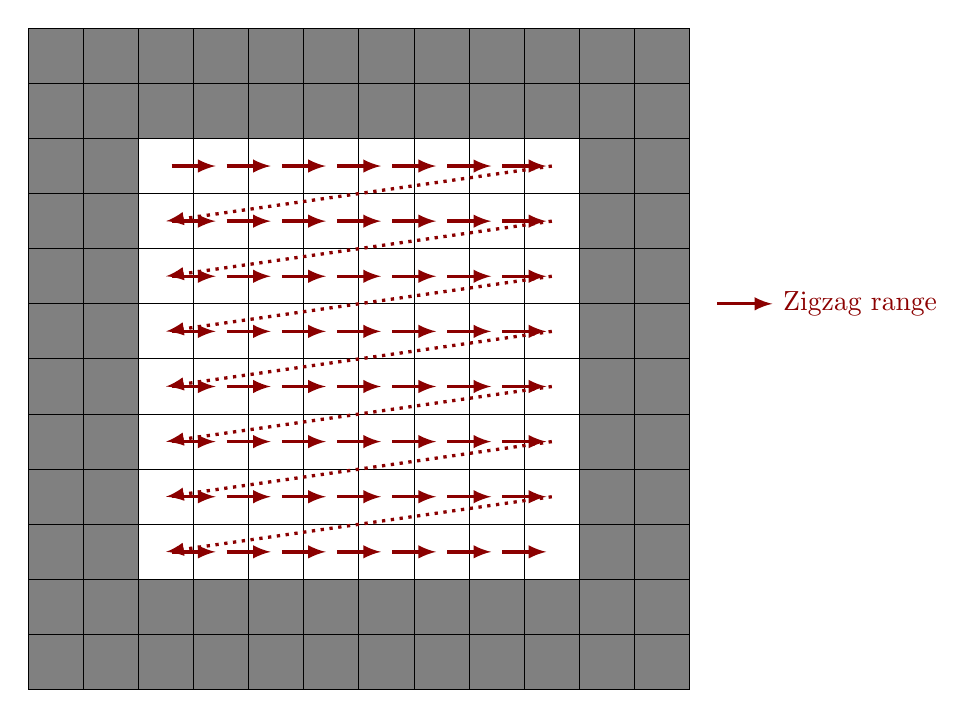
\begin{tikzpicture}[scale=.7,yscale=-1]
\tikzset{
  bg/.style={fill,gray},
  linear/.style={DarkRed,very thick,-latex}
}


\draw[bg] (0,0) rectangle (12,12);
\draw[fill=white] (2,2) rectangle (10,10);

\draw (0,0) grid[] (12,12);

\begin{scope}[shift={(.5,.5)}]
\foreach \y in {2, 3, ..., 8}{
  \foreach \x in {2, 3, ..., 8}
    \draw[linear] (\x+.1,\y) -- ++(.8,0);
  \draw[linear,dotted] (9,\y) -- (2,\y+1);
}
\foreach \x in {2, 3, ..., 8}
\draw[linear] (\x+.1,9) -- ++(.8,0);

\end{scope}

\begin{scope}[shift={(12.5,5)}]
\draw[linear,DarkRed] (0,0) -- ++(1,0) node[right] { Zigzag range };
\end{scope}


\end{tikzpicture}
\end{document}